% Self-contained Thompson-sampling diagram — compile with: pdflatex thompson.tex
% Output: thompson.pdf (single tightly-cropped page).
\documentclass[border=10pt]{standalone}
\usepackage{tikz}
\usepackage{amsmath, amssymb}
\usepackage{xcolor}

% --- Font-size compensation for down-scaled inclusion --------------------
% This diagram is included in the paper at a fraction of its natural width
% (see sec-design.tex), which shrinks every label. \small and \scriptsize are
% redefined here so that labels land near 8pt and tick marks near 6.5pt in the
% typeset paper. Re-tune if the \includegraphics width changes.
\usepackage{anyfontsize}
\renewcommand{\small}{\fontsize{15.3}{18.4}\selectfont}
\renewcommand{\scriptsize}{\fontsize{12.5}{15.0}\selectfont}
\usetikzlibrary{patterns}

% Palette (subdued, paper-style)
\definecolor{cInk}{HTML}{222222}
\definecolor{cMute}{HTML}{777777}
\definecolor{cAccent}{HTML}{2C4A6E}
\definecolor{cAccent2}{HTML}{B23A48}
\definecolor{cAccent2Soft}{HTML}{F0CCD0}

\begin{document}
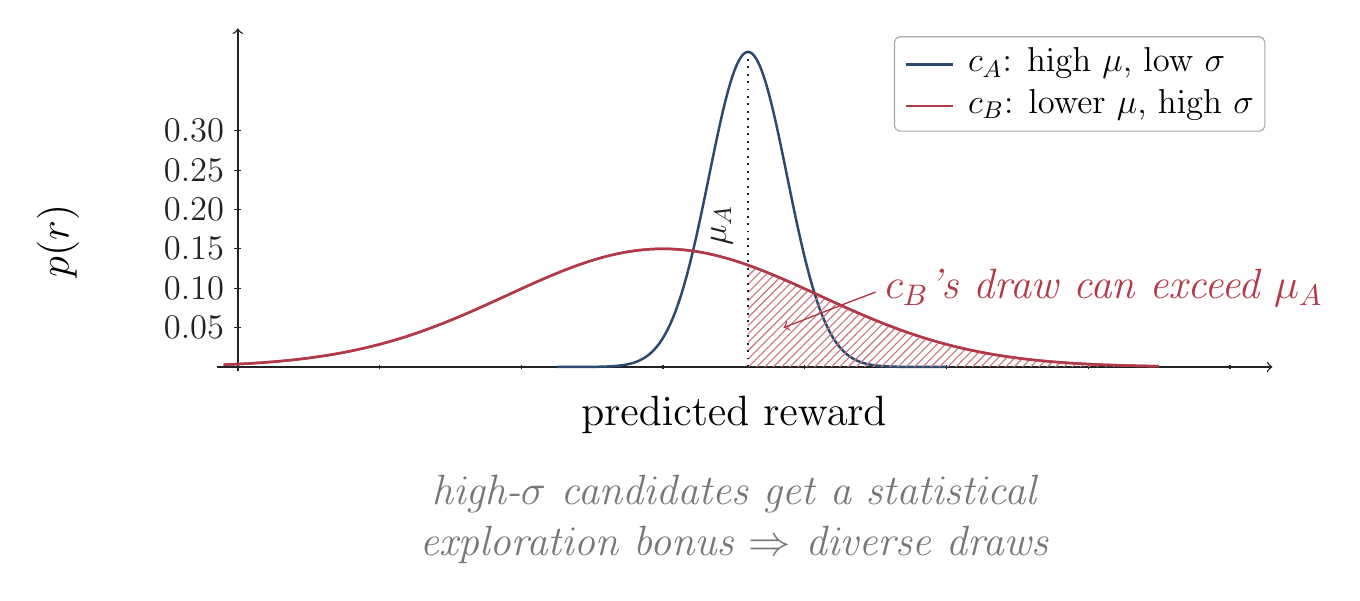
\begin{tikzpicture}[x=0.9cm, y=10cm]

  % Plot frame: x = predicted reward in [-4, 10], y = density in [0, 0.32]
  % Same geometry as cvar.tex / debiasing.tex.

  \draw[->, line width=0.5pt, color=cInk] (-4.3, 0)    -- (10.6, 0);
  \draw[->, line width=0.5pt, color=cInk] (-4.0,-0.005) -- (-4.0, 0.43);
  \node[font=\small, anchor=north] at (3.0, -0.025) {predicted reward};
  \node[font=\small, rotate=90, anchor=south] at (-6.10, 0.16) {$p(r)$};

  \foreach \y/\lab in {0.05/0.05, 0.10/0.10, 0.15/0.15, 0.20/0.20, 0.25/0.25, 0.30/0.30}{
    \draw[line width=0.4pt, color=cInk] (-4.05,\y) -- (-3.95,\y);
    \node[font=\scriptsize, color=cInk, anchor=east, xshift=-0.05cm] at (-4.0,\y) {\lab};
  }
  \foreach \x in {-4,-2,0,2,4,6,8,10}{
    \draw[line width=0.4pt, color=cInk] (\x,-0.003) -- (\x, 0.003);
  }

  % Two candidate ensemble posteriors:
  %   c_A (blue) : mu = 3.2, sigma = 0.55, peak amp 0.40  (greedy pick, sharper)
  %   c_B (red ) : mu = 2.0, sigma = 2.2,  peak amp 0.15  (high sigma)

  \draw[line width=0.9pt, color=cAccent, smooth, samples=200, domain=0.5:6.0]
        plot (\x, {0.40 * exp(-0.5*((\x-3.2)/0.55)^2)});

  \draw[line width=0.9pt, color=cAccent2, smooth, samples=240, domain=-4.2:9]
        plot (\x, {0.15 * exp(-0.5*((\x-2.0)/2.2)^2)});

  % Shaded right tail of c_B beyond mu_A = 3.2
  \begin{scope}
    \clip (3.2, 0) rectangle (9.0, 0.32);
    \fill[cAccent2Soft, pattern=north east lines, pattern color=cAccent2!70,
          smooth, samples=240, domain=3.2:9.0]
          plot (\x, {0.15 * exp(-0.5*((\x-2.0)/2.2)^2)})
          -- (9.0, 0) -- (3.2, 0) -- cycle;
  \end{scope}
  % re-stroke c_B
  \draw[line width=0.9pt, color=cAccent2, smooth, samples=240, domain=-4.2:9]
        plot (\x, {0.15 * exp(-0.5*((\x-2.0)/2.2)^2)});

  % Reference line at mu_A
  \draw[dotted, line width=0.7pt, color=cInk] (3.2, 0) -- (3.2, 0.40);
  \node[font=\scriptsize, color=cInk, rotate=90, anchor=south] at (3.12, 0.18)
        {$\mu_A$};

  % Annotation
  \node[font=\small\itshape, color=cAccent2, anchor=west, align=left] at (5.0, 0.10)
        {$c_B$'s draw can exceed $\mu_A$};
  \draw[->, line width=0.5pt, color=cAccent2] (5.0, 0.095) .. controls
        (4.4, 0.075) and (4.0, 0.06) .. (3.7, 0.05);

  \node[font=\small\itshape, color=cMute, anchor=north, align=center] at (3.0, -0.125)
        {high-$\sigma$ candidates get a statistical\\
         exploration bonus $\Rightarrow$ diverse draws};

  % Legend (top-right)
  \node[draw=cInk!40, line width=0.4pt, fill=white, rounded corners=2pt,
        inner sep=4pt, anchor=north east, align=left, font=\scriptsize]
        at (10.5, 0.42)
        {\textcolor{cAccent}{\rule[0.4ex]{1.4em}{0.9pt}}\;\,$c_A$: high $\mu$, low $\sigma$\\
         \textcolor{cAccent2}{\rule[0.4ex]{1.4em}{0.9pt}}\;\,$c_B$: lower $\mu$, high $\sigma$};

\end{tikzpicture}
\end{document}
